\documentclass{beamer}
\usepackage[T2A]{fontenc}
\usepackage[utf8]{inputenc}
\usepackage[english]{babel}
\usepackage{amssymb, amsfonts, amsmath, mathtext, cite, enumerate, float, indentfirst, graphicx, epstopdf, mathtools, color}

\usetheme{default}
\usecolortheme{default}

% Set up slides numbering
\makeatletter
\defbeamertemplate*{footline}{my theme}{
    \leavevmode
    \hbox{
    \begin{beamercolorbox}[wd = \paperwidth, ht = 5ex, dp = 4ex, right]{}
        \insertframenumber{} / \inserttotalframenumber\hspace*{5ex}
    \end{beamercolorbox}}
}
\makeatother


% Remove lower navigation panel
\setbeamertemplate{navigation symbols}{}

% Remove upper navigation panel (section/subsection)
\setbeamertemplate{headline}{}

% Reference numbers color
\setbeamercolor{footnote mark}{fg = red}

% Figures numbering
\setbeamertemplate{caption}[numbered]

\begin{document}

%% -TITLE-
\title{Symmetry breaking in competing single-well linear-nonlinear potentials}
\author{D.~A.~Zezyulin\inst{1}, \underline{M.~E.~Lebedev}\inst{2,3}, G.~L.~Alfimov\inst{2,4}, B.~A.~Malomed\inst{1,5}}
\institute{
	\inst{1} ITMO University, St. Petersburg, Russia \and
	\inst{2} Institute of Mathematics RAS, Ufa, Russia \and
	\inst{3} All-Russian Institute for Scientific and Technical Information RAS, Moscow, Russia \and
	\inst{4} MIEE University, Zelenograd, Moscow, Russia \and
	\inst{5} Faculty of Engineering, Tel Aviv University, Tel Aviv, Israel
} 
\date{20 Mar. 2019 \\ Bannoe, Magnitogorsk}
%% -END-


%% -SLIDE-
\begin{frame}[noframenumbering, plain]
\maketitle
\end{frame}
%% -END-


%% -SLIDE-
\begin{frame}
\frametitle{Setup}
One-dimentional Gross-Pitaevskii equation:
$$i\Psi_t = -\Psi_{xx} + V(x) \Psi - P(x) |\Psi|^2 \Psi, \quad V(x), P(x) \in \mathbb{R}.$$

{\bf Optics}: implanting nonlinearity-inducing dopants\footnotemark[1].

{\bf BEC}: locally applied Feshbach resonance\footnotemark[2].

\begin{itemize}
\item $V(x)$ -- linear potential;
\item $P(x)$ -- nonlinear (pseudo) potential.
\end{itemize}

\medskip

Stationary localized nonlinear modes: $\left\| \begin{array}{l} \Psi(t, x) = e^{-i \mu x} u(x) \\ \lim \limits_{x \to \infty} u(x) = 0 \end{array}\right.$

\footnotetext[1]{\footnotesize{J. Hukriede, D. Runde, and D. Kip, Phys. D {\bf 36}, R1-R16 (2003)}}
\footnotetext[2]{\footnotesize{D. M. Bauer, M. Lettner, C. Vo, G. Rempe and S. D\"urr, Nature Phys. 5, 339-342 (2009)}}
\end{frame}
%% -END-


%% -SLIDE-
\begin{frame}
\frametitle{SSB}

{\bf Spontaneous symmetry breaking (SSB)} --- type of bifurcation when one symmetric solution loses its stability and two stable asymmetric solutions arise.

\begin{figure}
\center{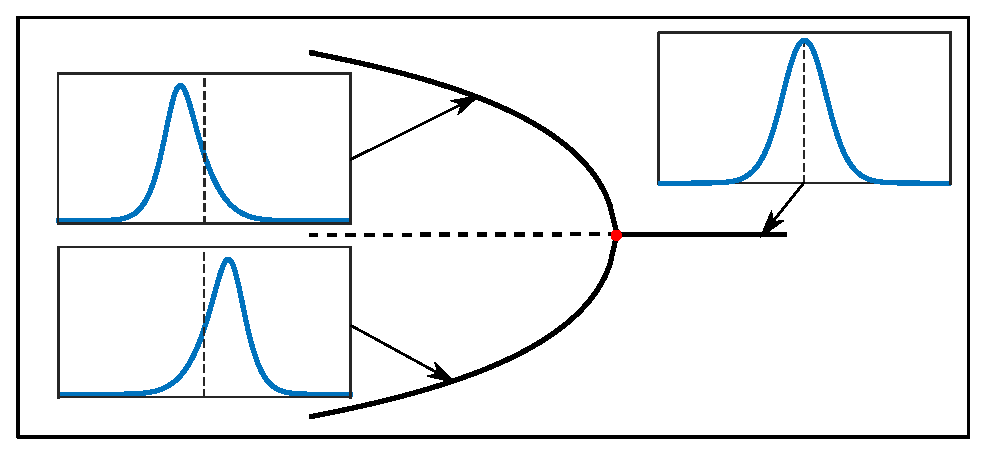
\includegraphics[width=1\textwidth]{pic/SSB_scheme.eps}}
\label{pic:ssb_scheme}
\end{figure}

\end{frame}
%% -END-


%% -SLIDE-
\begin{frame}
\frametitle{SSB: examples (1)}

GNLS (Generalized NLS), $V(x)$ -- double-well\footnotemark[3]:
$$i \Psi_t = -\Psi_{xx} + V(x) \Psi - |\Psi|^2 \Psi + 0.25 |\Psi|^4 \Psi.$$

\begin{figure}
\center{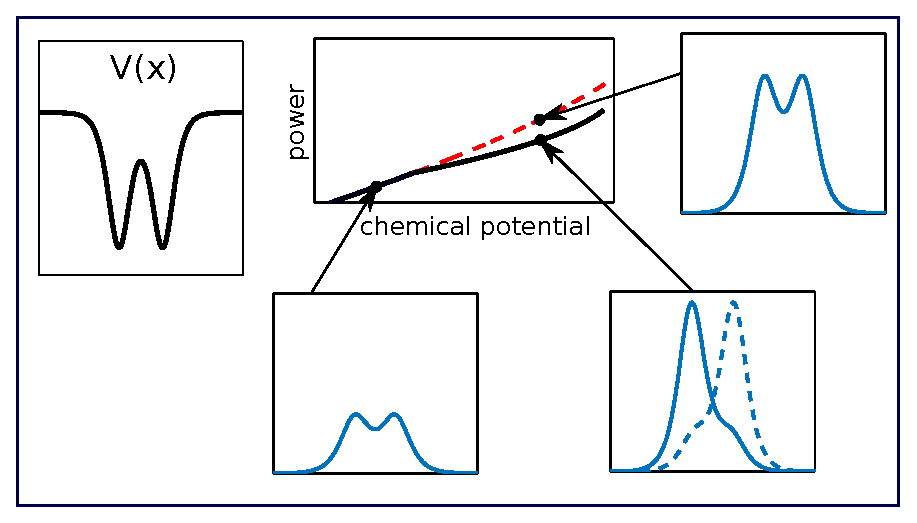
\includegraphics[width=1\textwidth]{pic/SSB_ex1.eps}}
\label{pic:ssb_ex1}
\end{figure}

\footnotetext[3]{\footnotesize{Jianke Yang, Phys. D {\bf 244}, 50-67 (2013)}}
\end{frame}
%% -SLIDE-


%% -SLIDE-
\begin{frame}
\frametitle{SSB: examples (2)}

2D GNLS, $V(x, y)$ -- double-well\footnotemark[3]:
$$i \Psi_t = -\Psi_{xx} - \Psi_{yy} + V(x, y) \Psi + |\Psi|^2 \Psi.$$

\begin{figure}
\center{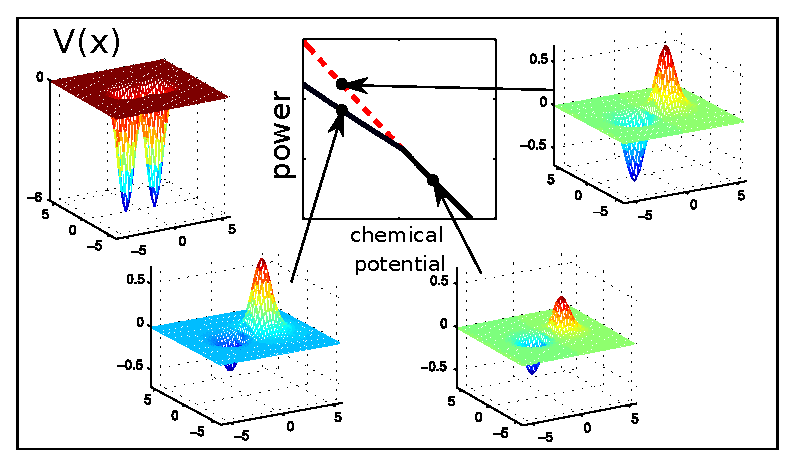
\includegraphics[width=1\textwidth]{pic/SSB_ex2.eps}}
\label{pic:ssb_ex2}
\end{figure}

\footnotetext[3]{\footnotesize{Jianke Yang, Phys. D {\bf 244}, 50-67 (2013)}}
\end{frame}
%% -END-


%% -SLIDE-
\begin{frame}
\frametitle{SSB: examples (3)}

NLS, $V(x) = 0$, $P(x)$ -- double-well\footnotemark[4]:
$$i \Psi_t = \Psi_{xx} + P(x) |\Psi|^2 \Psi.$$

\begin{figure}
\center{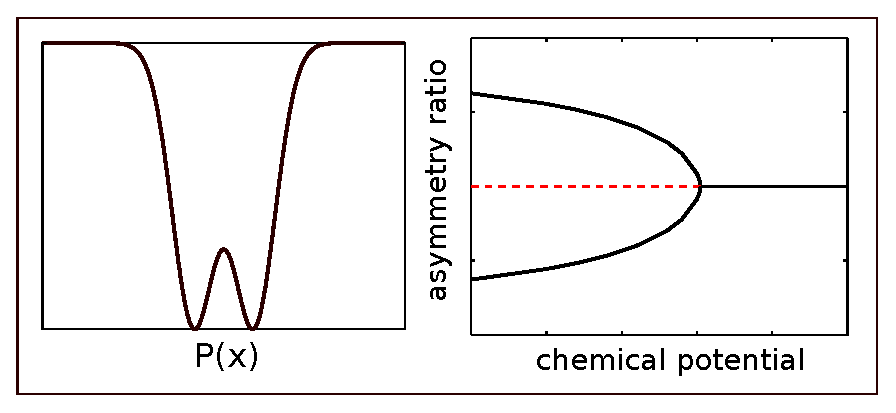
\includegraphics[width=1\textwidth]{pic/SSB_ex3.eps}}
\label{pic:ssb_ex3}
\end{figure}

\footnotetext[4]{\footnotesize{T. Mayteevarunyoo, B. A. Malomed, and G. Dong, Phys. Rev. A {\bf 78}, 053601 (2008)}}
\end{frame}
%% -END-


%% -SLIDE-
\begin{frame}
\frametitle{SSB without double-well structure?}
$$i\Psi_t = -\Psi_{xx} + V(x) \Psi - P(x) |\Psi|^2 \Psi;$$
\begin{center}
$V(x) = \dfrac{1}{2} \omega^2 x^2,$ \quad $P(x) = 1 + A \tanh^2{x}.$
\end{center}

\begin{figure}
\center{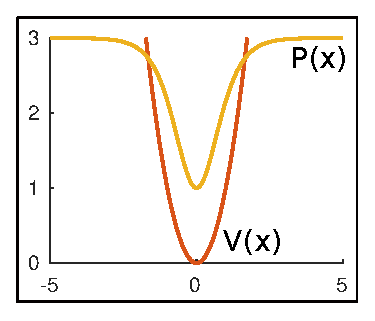
\includegraphics[scale=1]{pic/potentials.eps}}
\label{pic:potentials}
\end{figure}

\begin{center}
Interplay between linear and nonlinear potentials?
\end{center}
\end{frame}
%% -END-


%% -SLIDE-
\begin{frame}
\frametitle{$(\gamma_+, \gamma_-)$ diagrams\footnotemark[5]}
\begin{equation}
u_{xx} + (\mu - V(x)) u + P(x) u^3 = 0;
\label{eq:stationary}
\end{equation}

\begin{center}
$S_+ = \{u(x) | \lim \limits_{x \to +\infty} u(x) = 0\}$; \quad $u(x) \sim C_+ x^{\frac{1}{2}(\mu - 1)} e^{-\frac{\omega^2 x^2}{4}}$.
\end{center}

\begin{figure}
\center{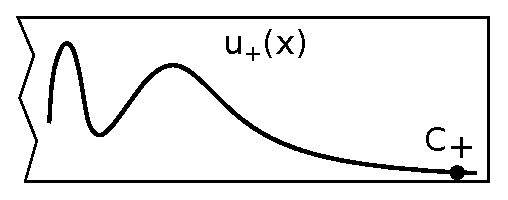
\includegraphics[scale=1]{pic/right_asymtotic.eps}}
\label{pic:right_asymptotic}
\end{figure}


\footnotetext[5]{\footnotesize{G. L. Alfimov and D. A. Zezyulin, Nonlinearity {\bf 20}, 2075–2092 (2007)}}
\end{frame}
%% -END-


%% -SLIDE-
\begin{frame}
\frametitle{$(\gamma_+, \gamma_-)$ diagrams}

\begin{center}
$S_- = \{u(x) | \lim \limits_{x \to -\infty} u(x) = 0\}$; \quad $u(x) \sim C_- (-x)^{\frac{1}{2}(\mu - 1)} e^{-\frac{\omega^2 x^2}{4}}$
\end{center}

\begin{figure}
\center{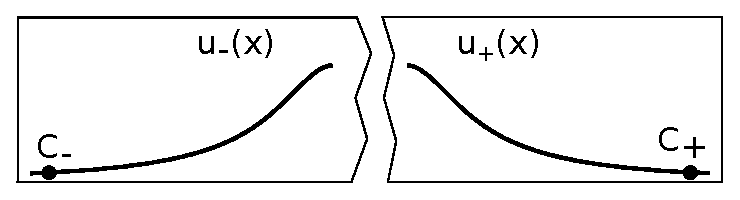
\includegraphics[width=1\textwidth]{pic/asymtotic.eps}}
\label{pic:asymptotic}
\end{figure}

\begin{center}
$u(x)$ -- localized \quad $\leftrightarrow$ \quad $u(x) \in S_+ \cap S_-$;
$u(0) = u_+(0; C_+) = u_-(0; C_-)$, \quad $u'(0) = u_+'(0; C_+) = u_-'(0; C_-)$.
\end{center}

\end{frame}
%% -END-


%% -SLIDE-
\begin{frame}
\frametitle{$(\gamma_+, \gamma_-)$ diagrams}

$\gamma_+ = \{ (u_+(0; C_+); u_+'(0; C_+)), \quad C_+ \in [-\tilde{C}_+, \tilde{C}_+] \}$;

$\gamma_- = \{ (u_-(0; C_-); u_-'(0; C_-)), \quad C_- \in [-\tilde{C}_-, \tilde{C}_-] \}$

\begin{figure}
\center{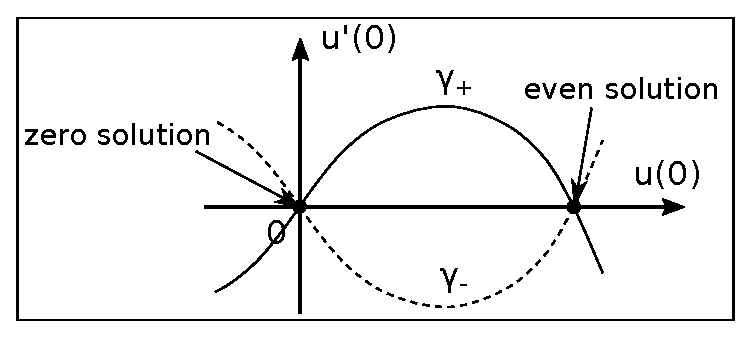
\includegraphics[scale=0.7]{pic/diagram.eps}}
\label{pic:diagram}
\end{figure}

Properties:
\begin{itemize}
\item each point of intersection $\gamma_+ \cap \gamma_-$ corresponds to a solution;
\item symmetry of equation $x \to -x$ leads to a symmetry of $\gamma_\pm$ curves about $u'$ axis;
\item intersections of $\gamma_\pm$ with $u$, $u'$ axes correspond to even and add localized modes.
\end{itemize}

\end{frame}
%% -END-


%% -SLIDE-
\begin{frame}
\frametitle{Application: $\mu = 0$, $A = 2$}

\begin{figure}
\center{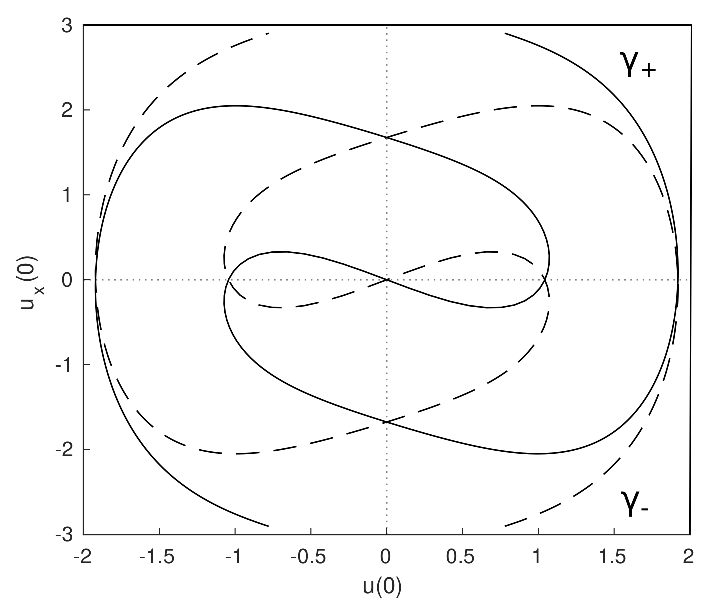
\includegraphics[width=0.9\textwidth]{pic/diagram_ex1.eps}}
\label{pic:diagram_ex1}
\end{figure}

\end{frame}
%% -END-


%% -SLIDE-
\begin{frame}
\frametitle{Application: $\mu = 0$, $A = 2$}

\begin{figure}
\center{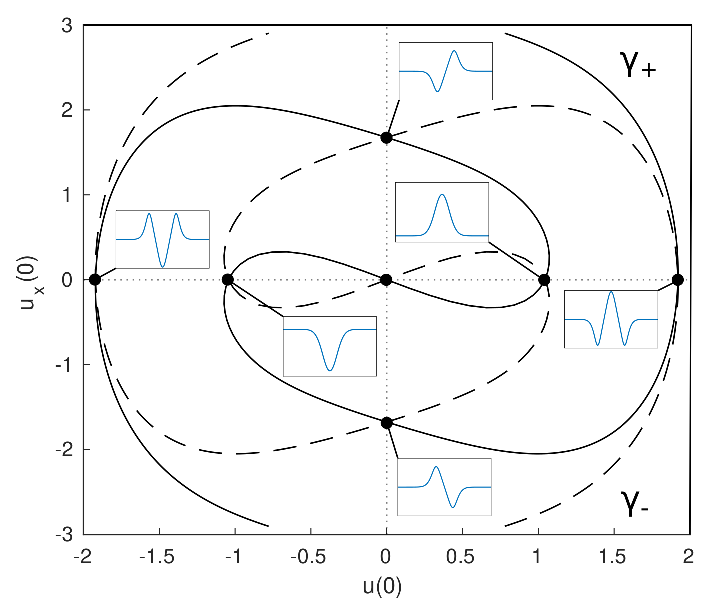
\includegraphics[width=0.9\textwidth]{pic/diagram_ex2.eps}}
\label{pic:diagram_ex2}
\end{figure}

\end{frame}
%% -END-


%% -SLIDE-
\begin{frame}
\frametitle{Application: $\mu = 0$, $A = 2$}

\begin{figure}
\center{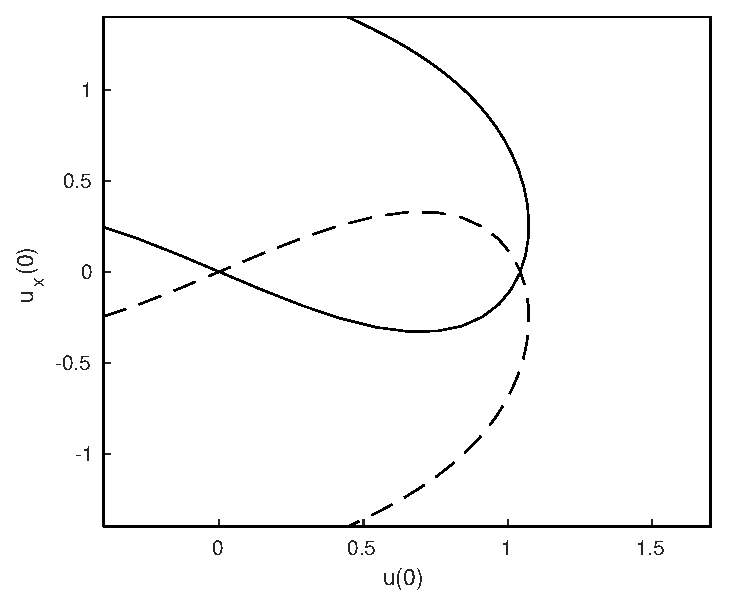
\includegraphics[width=0.9\textwidth]{pic/diagram_step_0.eps}}
\label{pic:diagram_step_0}
\end{figure}

\end{frame}
%% -END-


%% -SLIDE-
\begin{frame}
\frametitle{Application: $\mu = -0.5$, $A = 2$}

\begin{figure}
\center{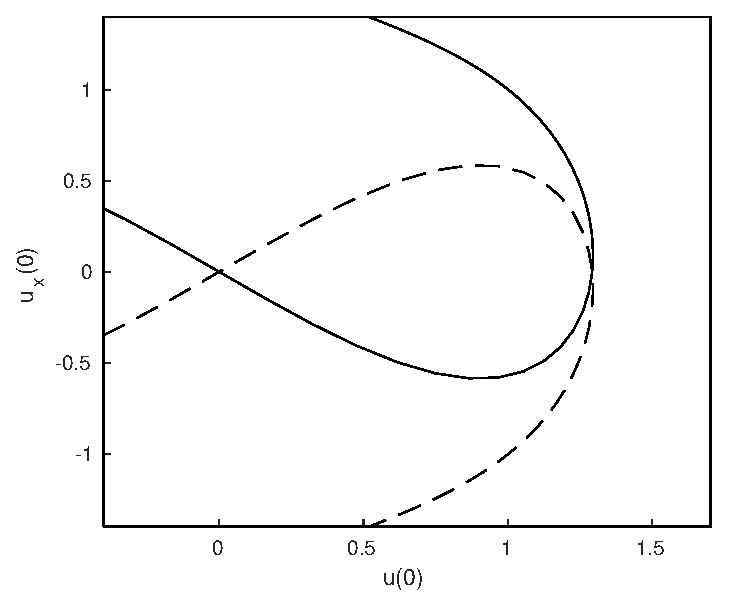
\includegraphics[width=0.9\textwidth]{pic/diagram_step_1.eps}}
\label{pic:diagram_step_1}
\end{figure}

\end{frame}
%% -END-


%% -SLIDE-
\begin{frame}
\frametitle{Application: $\mu = -0.8$, $A = 2$}

\begin{figure}
\center{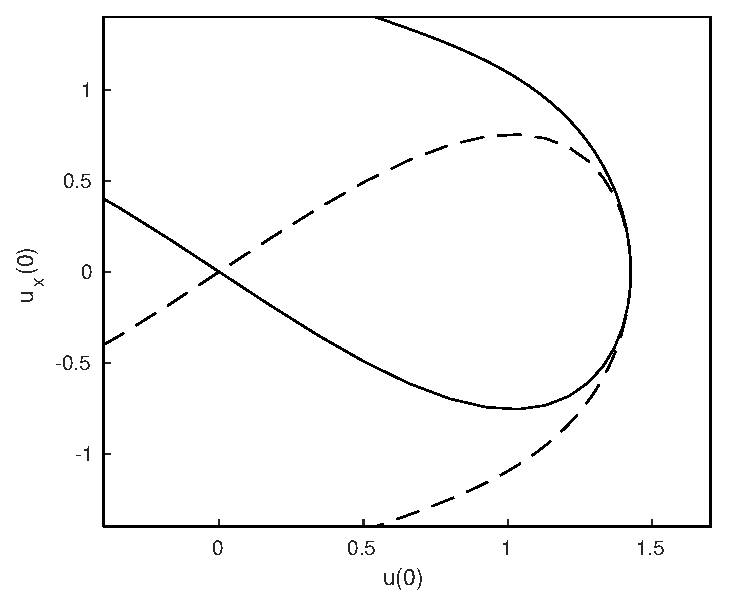
\includegraphics[width=0.9\textwidth]{pic/diagram_step_2.eps}}
\label{pic:diagram_step_2}
\end{figure}

\end{frame}
%% -END-


%% -SLIDE-
\begin{frame}
\frametitle{Application: $\mu = -1.1$, $A = 2$}

\begin{figure}
\center{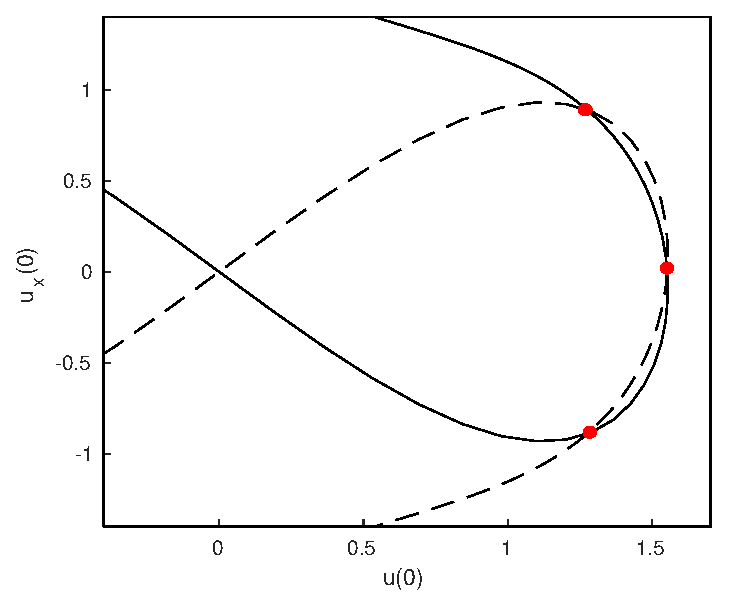
\includegraphics[width=0.9\textwidth]{pic/diagram_step_3.eps}}
\label{pic:diagram_step_3}
\end{figure}

\end{frame}
%% -END-


%% -SLIDE-
\begin{frame}
\frametitle{SSB bifurcation?}

\begin{figure}
\center{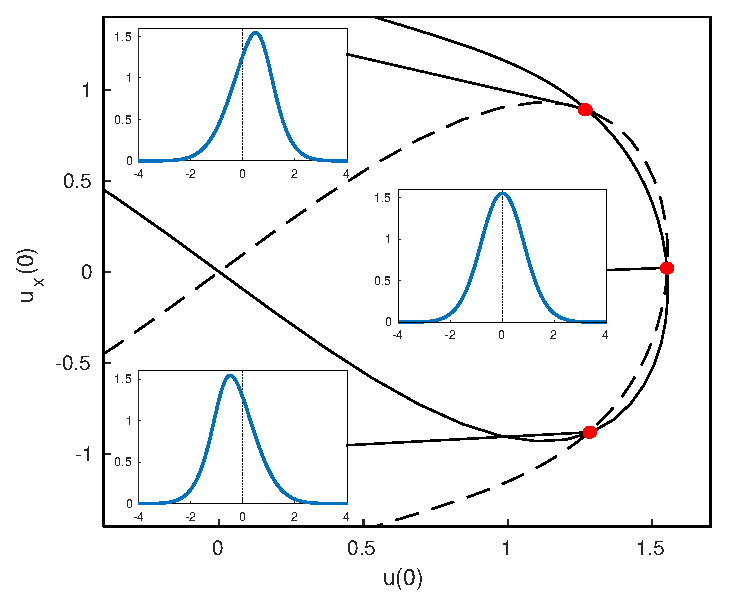
\includegraphics[width=0.9\textwidth]{pic/diagram_ssb.eps}}
\label{pic:diagram_ssb}
\end{figure}

\end{frame}
%% -END-


%% -SLIDE-
\begin{frame}
\frametitle{Stability}
Considering eqigenvalue problem for operator\footnotemark[5]:
\begin{equation}
\mathcal{L} = i \begin{pmatrix} 0 & \mathcal{L}_- \\ \mathcal{L}_+ & 0 \end{pmatrix}
\end{equation}
where $\mathcal{L}_\pm = \dfrac{d^2}{dx^2} + \mu - \dfrac{1}{2} \omega^2 x^2 + + (2 \pm 1) P(x) u^2$.

\begin{figure}
\center{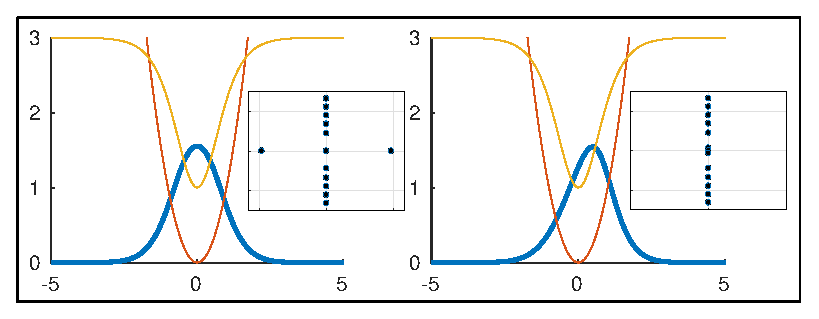
\includegraphics[width=0.8\textwidth]{pic/stability.eps}}
\label{pic:stability}
\end{figure}

\footnotetext[6]{\footnotesize{Jianke Yang, Nonlinear Waves in Integrable and Nonintegrable Systems, Society of Industrial and Applied Mathematics (2010)}}
\end{frame}
%% -END-


%% -SLIDE-
\begin{frame}
\frametitle{SSB bifurcation}

$$N = \int \limits_{-\infty}^{+\infty} u^2(x) dx, \quad X_c = N^{-1} \int \limits_{\infty}^{+\infty} x u^2(x) fx$$

\begin{figure}
\center{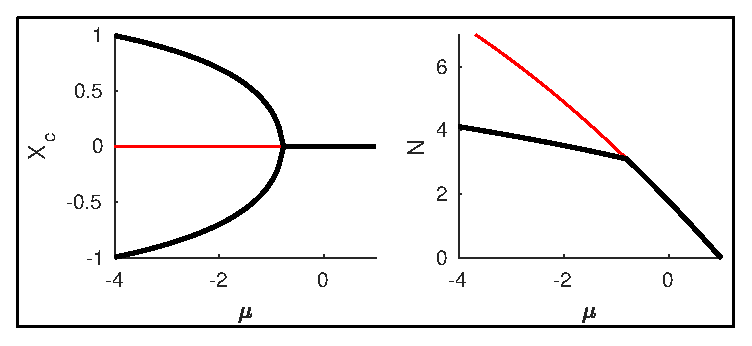
\includegraphics[width=0.8\textwidth]{pic/pitchfork.eps}}
\label{pic:pitchfork}
\end{figure}

\end{frame}
%% -END-


%% -SLIDE-
\begin{frame}
\frametitle{Evolution of unstable symmetric mode}
We use conservative Trofimov-Peskov finite-difference scheme\footnotemark[7] to calculate time evolution of the nonlinear modes.
\begin{figure}
\center{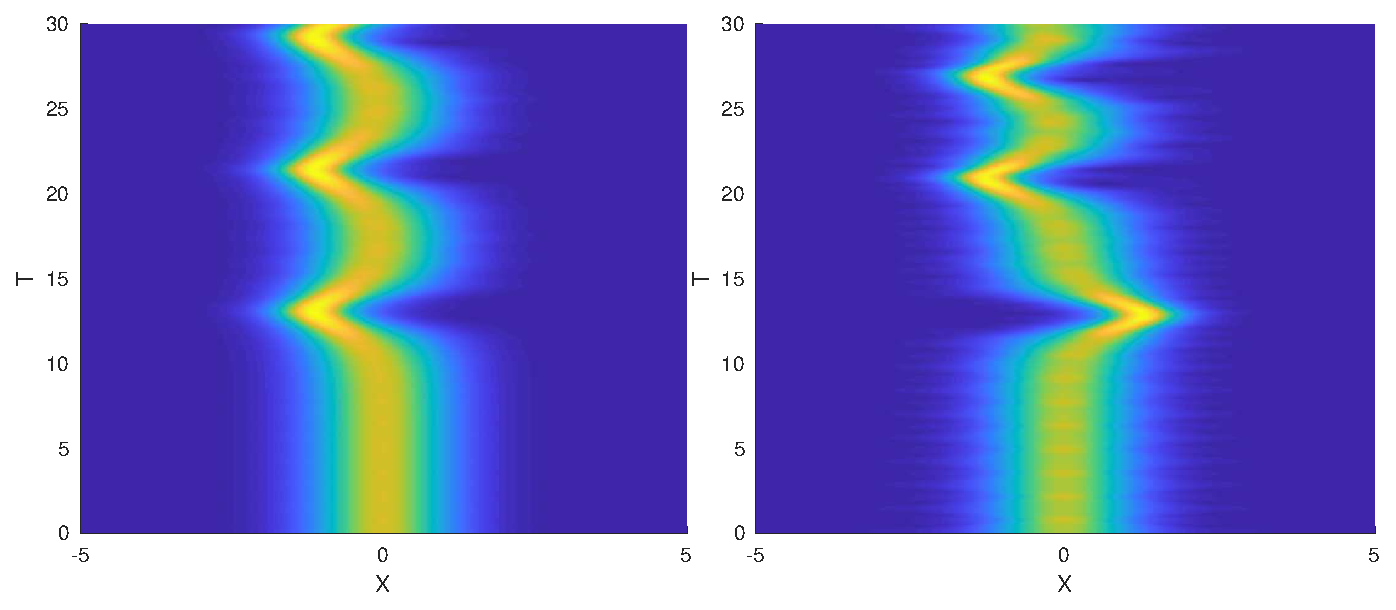
\includegraphics[width=\textwidth]{pic/evolution.eps}}
\label{pic:evolution}

\footnotetext[7]{\footnotesize{V. A. Trofimov, N. V. Peskov, Mathematical Modelling and Analysis, Volume 14 Number 1, 2009, pages 109-126}}
\end{figure}

\end{frame}
%% -END-


%% -SLIDE-
\begin{frame}
\frametitle{Unbounded nonlinear potential}

$$V(x) = \dfrac{1}{2} \omega^2 x^2; \quad P(x) = 1 + A x^2$$

\begin{figure}
\center{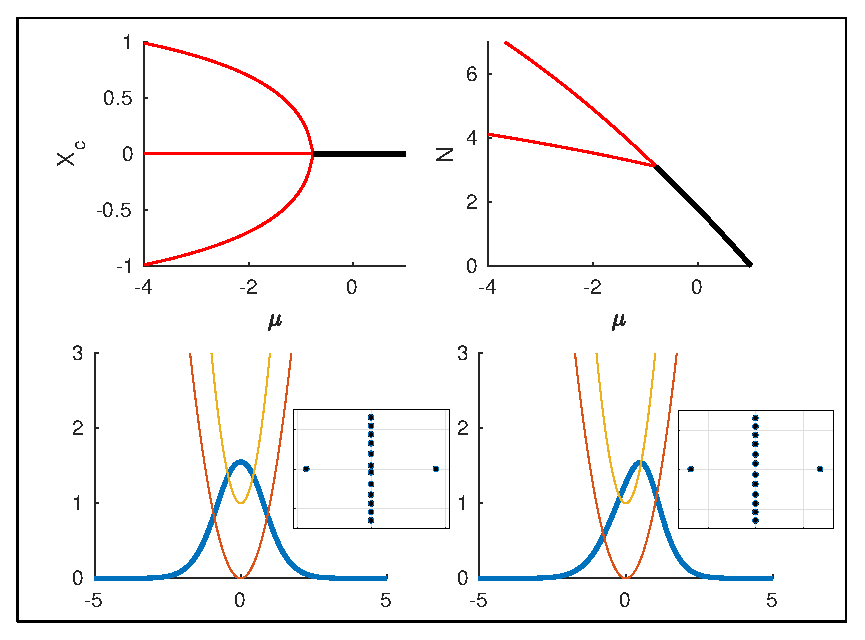
\includegraphics[width=0.85\textwidth]{pic/bifurcation_unbounded.eps}}
\label{pic:bifurcation_unbounded}
\end{figure}

\end{frame}
%% -END-


%% -SLIDE-
\begin{frame}
\frametitle{Conclusion}
\begin{itemize}
\item GPE equation with {\color{red} signle-well} linear and nonlinear potentials was considered:
$$i\Psi_t = -\Psi_{xx} + V(x) \Psi - P(x) |\Psi|^2 \Psi, \quad V(x), P(x) \in \mathbb{R}.$$
\item Method of $(\gamma_+, \gamma_-)$ diagrams helps us to understand the structure of nonlinear modes for this case.
\item SSB bifurcation was found. 
\end{itemize}
\end{frame}
%% -END-


%% -SLIDE-
\begin{frame}
\begin{figure}
\center{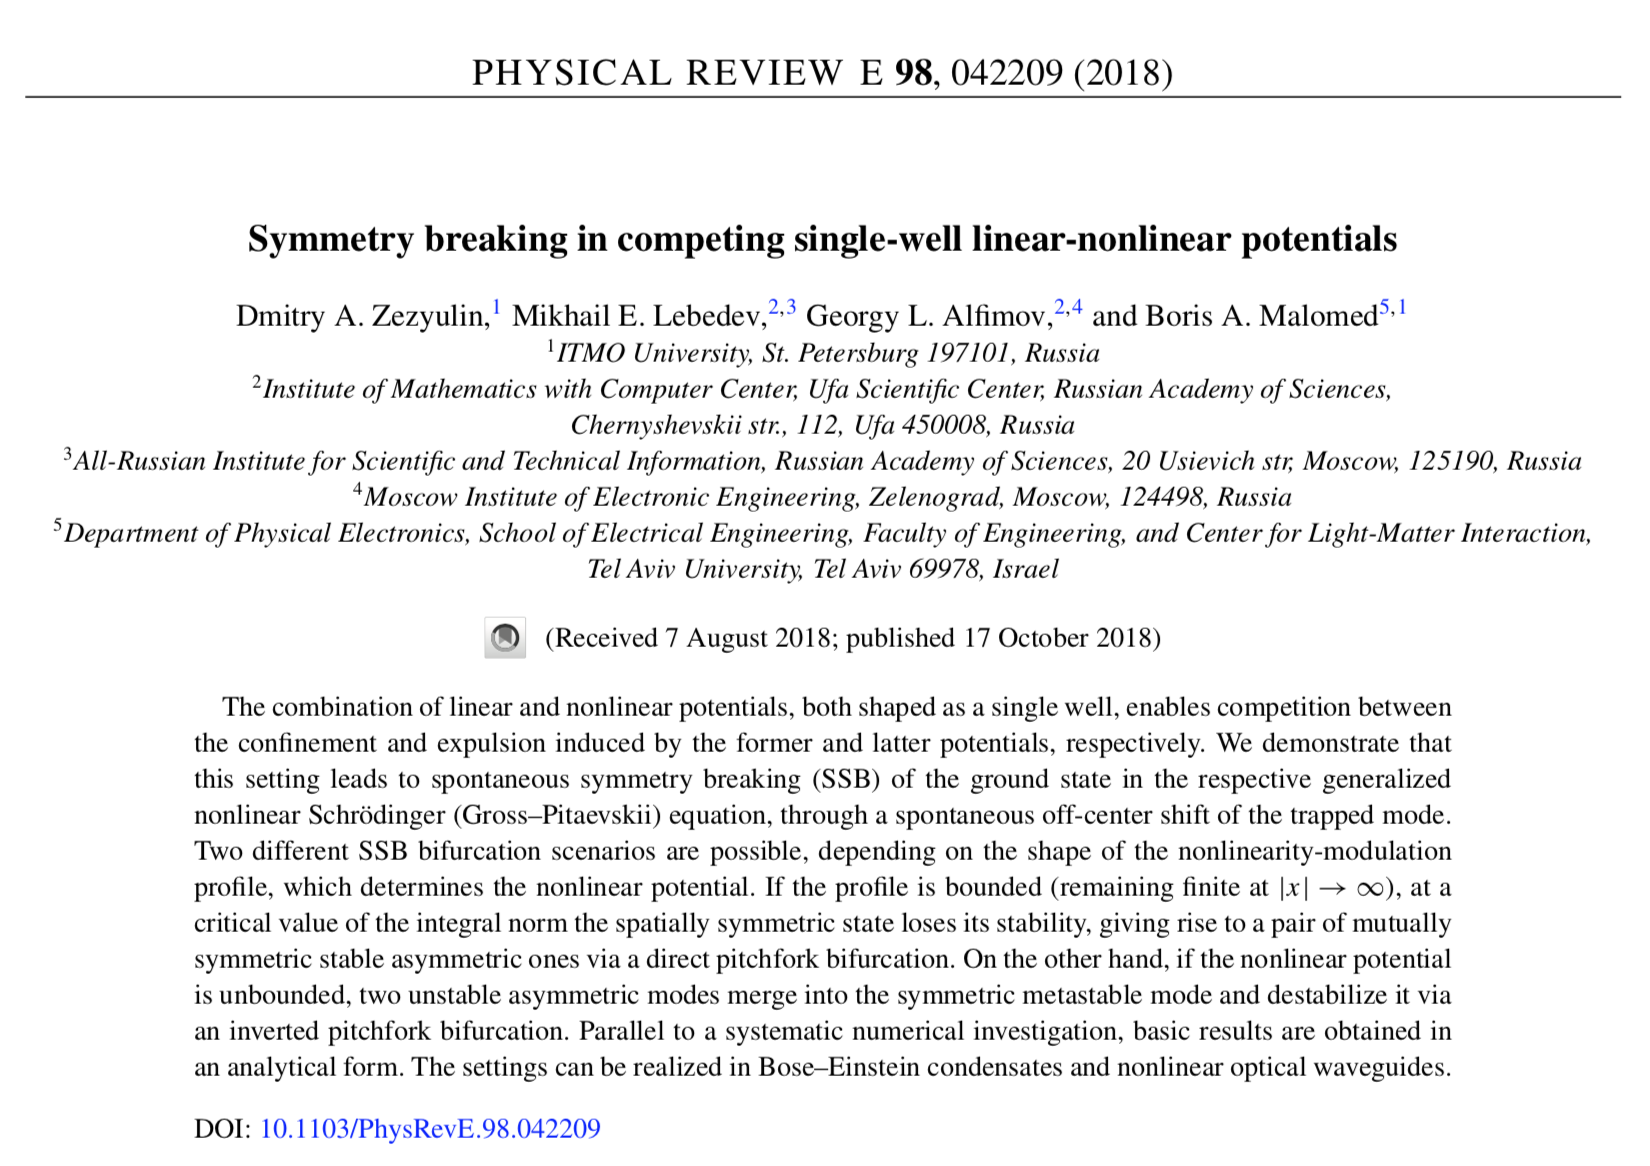
\includegraphics[width=\textwidth]{pic/publication.png}}
\label{pic:publication}
\end{figure}

\footnotetext[8]{\footnotesize{D. A. Zezyulin, M. E. Lebedev, G. L. Alfimov, and Boris A. Malomed, Phys. Rev. E {\bf 98}, 042209 (2018)}}
\end{frame}
%% -END-


%% -SLIDE-
\begin{frame}
\begin{center}
Thanks for your attention!
\end{center}
\end{frame}
%% -END-


\end{document}